\documentclass[conference]{IEEEtran}
\IEEEoverridecommandlockouts

\usepackage{cite}
\usepackage{amsmath,amssymb}
\usepackage{graphicx}
\usepackage{booktabs}
\usepackage{multirow}
\usepackage{array}
\usepackage{xcolor}
\usepackage{tikz}
\usetikzlibrary{arrows.meta,positioning,fit,backgrounds}
\usepackage[hidelinks]{hyperref}
\usepackage{url}

\graphicspath{{figures/}{screens/}}
\newcommand{\dAUC}{$\Delta$AUC}
\newcommand{\tierC}{Tier~C}
\newcommand{\tierE}{Tier~E}

\begin{document}

\title{Stream-Aware, Leakage-Safe Build Failure Prediction for Continuous Integration:\\
Pre-Registered Evidence from Travis~CI and GitHub Actions}

\author{\IEEEauthorblockN{Author Name}
\IEEEauthorblockA{Department, University\\
City, Country\\
email@example.com}}

\maketitle

\begin{abstract}
Predicting which continuous integration (CI) builds will fail lets teams spend a fixed review budget where it matters, but published results are easy to inflate: post-build fields leak the outcome, random train/test splits let the future predict the past, and pooled metrics reward telling repositories apart rather than ranking a repository's own builds. We study build failure prediction under a strict protocol: only information available when a build is triggered, history that counts a prior build only once it has \emph{finished}, chronological walk-forward evaluation, and macro \emph{within-repository} AUC with paired repository-bootstrap confidence intervals. On 858{,}368 Travis~CI builds from 947 projects, a leakage-safe Random Forest with repository history (\tierC) reaches 0.628 within-repository AUC, far below the 0.91 a random split suggests. Adding history for the build's own \emph{stream} (its pull request or branch), in-flight context, and a learning-to-rank objective (\tierE) raises this to 0.698 (+0.070, every fold's 95\% CI above zero), including +0.066 on \emph{new breakages}. We then tested the frozen recipe on GitHub Actions under protocols hashed before data collection: on 30 repositories the gain replicated in direction (+0.055) but was inconclusive under the pre-registered rule; on 30 \emph{new} repositories it was confirmed (0.911 vs.\ 0.763, +0.149, 5 of 5 folds). We deploy the model behind a GitHub webhook that scores each workflow run when it is requested, with a per-repository 15\% review budget, and release a read-only public demonstration. A forward-looking test of the frozen deployed system is pre-registered.
\end{abstract}

\begin{IEEEkeywords}
continuous integration, build failure prediction, data leakage, learning to rank, pre-registration, GitHub Actions, software analytics
\end{IEEEkeywords}

%=====================================================================
\section{Introduction}
%=====================================================================

Continuous integration (CI) runs a project's build and tests on every push and pull request~\cite{hilton2016usage}. Failed builds cost developer attention and compute, and a large literature asks whether failures can be predicted before a build runs~\cite{hassan2017change,ni2017cost,xia2017could,chen2020buildfast,jin2020cost}. A useful predictor would let a team review, prioritise, or defer the riskiest builds within a fixed budget.

Reported accuracy in this area is often optimistic for three avoidable reasons. First, \emph{leakage}~\cite{kaufman2012leakage}: CI datasets such as TravisTorrent~\cite{beller2017travistorrent} mix pre-build fields with fields computed from the build log, such as test counts and durations, that encode the outcome. Second, \emph{random splits}: when builds are shuffled, models learn a repository's future failure rate and use it to predict its past~\cite{bergmeir2012use}. Third, \emph{pooled metrics}: repositories differ widely in failure rate, so a model can earn a high pooled AUC simply by recognising risky repositories, which says little about ranking a single team's builds, the decision a team actually faces.

This paper makes the following contributions:
\begin{itemize}
\item A \textbf{leakage-safe protocol} for build failure prediction: an availability registry enforced at training and inference time, finish-time-safe history, chronological walk-forward folds, and macro within-repository AUC with paired repository-bootstrap CIs. We quantify how much the shortcuts inflate results on TravisTorrent (Section~\ref{sec:leakage}).
\item \textbf{\tierE}, a model that adds history for the build's own \emph{stream} (pull request or branch), in-flight context, and a learning-to-rank objective. It improves within-repository AUC from 0.628 to 0.698 on Travis~CI, and the gain holds on new breakages (Section~\ref{sec:results}).
\item Two \textbf{pre-registered external tests} on GitHub Actions. The first replicated in direction but was inconclusive under its rule; a confirmation on 30 new repositories met it decisively (Section~\ref{sec:gha}).
\item A \textbf{deployed system}, with live history verified identical to the training pass, alerts issued under a per-repository review budget that matches the evaluation metric, and a read-only public demonstration (Section~\ref{sec:system}).
\item A \textbf{pre-registered forward-looking test} of the frozen deployed system on data that did not exist when it was frozen (Section~\ref{sec:prospective}).
\end{itemize}

%=====================================================================
\section{Related Work}
%=====================================================================

\textbf{CI practice and failures.} Hilton et al.\ document CI's costs and benefits in open source~\cite{hilton2016usage}; Rausch et al.\ characterise build failure causes~\cite{rausch2017empirical}. TravisTorrent~\cite{beller2017travistorrent} made Travis~CI build histories widely available, and later studies flag noise and heterogeneity in such data~\cite{gallaba2018noise,durieux2019analysis}.

\textbf{Build outcome prediction.} Hassan and Wang predict build outcomes from change features~\cite{hassan2017change}; Ni and Li use cascaded classifiers to cut cost~\cite{ni2017cost}; Xia and Li compare learners~\cite{xia2017could}. BuildFast~\cite{chen2020buildfast} adds history-aware features, and Jin and Servant study cost-efficient build selection~\cite{jin2020cost}. Common to most of this work are pooled metrics and splits or history features that ignore build finish times; history that ignores finish times can include builds that had not finished when the current build was triggered.

\textbf{Methodology.} We follow the leakage taxonomy of Kaufman et al.~\cite{kaufman2012leakage} and time-respecting evaluation~\cite{bergmeir2012use}, use bootstrap CIs~\cite{efron1993introduction}, and adopt pre-registration~\cite{nosek2018preregistration} to keep confirmatory tests honest. The models use Random Forests~\cite{breiman2001random}, LightGBM~\cite{ke2017lightgbm} with the XE-NDCG ranking loss~\cite{bruch2021alternative}, Platt scaling~\cite{platt1999probabilistic}, and SHAP explanations~\cite{lundberg2017unified}.

%=====================================================================
\section{Data}
%=====================================================================

Table~\ref{tab:data} summarises the three datasets.

\textbf{Travis~CI.} The TravisTorrent export~\cite{beller2017travistorrent} has 3.56M job rows. We collapse them to \textbf{858{,}368 builds} from \textbf{947 projects} (April~2011 to August~2016), asserting that every pre-build field is constant across a build's jobs. A build fails if any of its jobs failed (19.5\% of builds). A build's finish time is its start time plus its longest job's duration, with a per-repository 95th-percentile fallback for missing durations.

\textbf{GitHub Actions.} The unit is a workflow run. We keep first attempts of \texttt{push} and \texttt{pull\_request} runs; \texttt{success} is a pass, and \texttt{failure} and \texttt{startup\_failure} are failures. A run's finish time is its \texttt{updated\_at}, and runs whose completion time is unknown (over 35 days) are dropped. Commit size comes from the commits API. The \emph{first} dataset has 67{,}980 runs from 30 repositories (2025--26, 8.9\% failures). The \emph{confirmation} dataset was collected under its own pre-registered protocol: the first 30 eligible repositories from a star-sorted search, excluding every repository used before, with runs created from 15~August to 30~September~2026. That gives 78{,}576 runs (28.2\% failures) after dropping 3{,}773 runs (4.6\%) whose fork commits could no longer be fetched.

\begin{table}[t]
\caption{Datasets. ``Failure rate'' is per build or run.}
\label{tab:data}
\centering
\footnotesize
\setlength{\tabcolsep}{4pt}
\begin{tabular}{@{}lrrrl@{}}
\toprule
Dataset & Units & Repos & Fail.\ rate & Period \\
\midrule
Travis~CI (TravisTorrent) & 858{,}368 & 947 & 19.5\% & 2011--2016 \\
GHA test 1 & 67{,}980 & 30 & 8.9\% & 2025--2026 \\
GHA confirmation & 78{,}576 & 30 & 28.2\% & Aug--Sep 2026 \\
GHA combined & 146{,}556 & 60 & 19.2\% & 2025--2026 \\
\bottomrule
\end{tabular}
\end{table}

%=====================================================================
\section{A Leakage-Safe Problem Setup}
\label{sec:leakage}
%=====================================================================

\textbf{Availability registry.} Every column is recorded in a versioned registry with the stage at which it becomes known: pre-build, build start, or post-build. The predictor refuses to start if any model input is not marked available at prediction time, so leaky fields cannot re-enter by accident. Fields such as \texttt{tr\_log\_*} test counts, durations, and comment counts that may be written after the build are blocked.

\textbf{Finish-time-safe history.} A prior build contributes its outcome to a new build's history only if it \emph{finished} strictly before the new build was triggered. Ties are ordered by finish time, trigger time, then build id. A brute-force recomputation re-checks the history values on sampled repositories in every run, and a deliberately leaked feature makes it fail. Optional \emph{finish buffers} of 1~h and 6~h delay each outcome further.

\textbf{How much the shortcuts inflate results.} Table~\ref{tab:leakage} shows the same family of models under progressively stricter setups. On a random split, adding post-build fields lifts AUC from 0.690 to 0.896. Even without leaky fields, the random-split AUC of a 39-feature model with repository history (0.91) falls to 0.82 on a chronological split and to 0.63 when measured \emph{within} repositories at the build level. That last setup is the one that matches a team's decision, and it is the one we report.

\begin{table}[t]
\caption{The same task under progressively stricter setups (Travis~CI).}
\label{tab:leakage}
\centering
\footnotesize
\setlength{\tabcolsep}{4pt}
\begin{tabular}{@{}p{4.9cm}r@{}}
\toprule
Setup & AUC \\
\midrule
Random split, 31 features incl.\ post-build log fields & 0.896 \\
Random split, 13 strict pre-build features & 0.690 \\
Random split, 39 features with repository history (stacking) & 0.912 \\
Chronological split, job level, pooled (RF) & 0.821 \\
Walk-forward, build level, \emph{within-repo} (\tierC\ RF) & 0.628 \\
\bottomrule
\end{tabular}
\end{table}

%=====================================================================
\section{Method}
%=====================================================================

\subsection{Feature tiers}
\textbf{Tier~A} holds 18 change and context features known at trigger time: source and test churn, files added, deleted and modified by type, time of day and week, pull request flag, core-team author, and default branch, plus the language. \textbf{\tierC} adds project context documented by TravisTorrent (team size, code size, test density, past commits on the touched files, commits in the build) and repository history: the previous finished build's outcome and the repository's last-5 and overall failure rates. On GitHub Actions the change features are the head commit's additions, deletions, files changed, message length and parents, with the workflow as a categorical feature.

\textbf{\tierE} adds two groups. \emph{Stream history}: a stream is the build's pull request (on GitHub Actions, the PR author and head branch, since runs carry no PR number) or, for push builds, its branch. Stream features are the outcome of the stream's last finished build, its last-5 and overall failure rates, its count of finished builds and failure streak, the outcome of the build's predecessor (on Travis, the previous build on the branch; on GitHub Actions, the previous run of the same workflow on the stream), and an exponentially weighted repository failure rate. \emph{In-flight context} records whether the previous build and the stream's last build are still running, how many repository builds are running, how many started in the last hour, and the hours since the stream last triggered. In-flight features use only the existence and start times of earlier builds, never their outcomes.

\subsection{Model}
Within-repository ranking is the goal, so \tierE\ combines a binary LightGBM classifier~\cite{ke2017lightgbm} with a LightGBM ranker trained with the XE-NDCG objective~\cite{bruch2021alternative}. Each ranking query is one repository's builds in one calendar month. Let $b(x)$ be the classifier's log-odds and $r(x)$ the ranker's score. Both are standardised with \emph{training-score} moments and averaged,
\begin{equation}
s(x) = \tfrac{1}{2}\,\frac{r(x)-\mu_r}{\sigma_r} + \tfrac{1}{2}\,\frac{b(x)-\mu_b}{\sigma_b},
\end{equation}
and one global Platt map~\cite{platt1999probabilistic}, fitted on training scores, turns $s(x)$ into a probability. Hyperparameters were fixed before any confirmation fold was scored. Explanations use SHAP values~\cite{lundberg2017unified} of the binary half.

%=====================================================================
\section{Evaluation Protocol}
%=====================================================================

\textbf{Walk-forward folds.} Builds are sorted by trigger time and split into 10 equal chronological folds. Fold $k$ is tested after training on folds $1,\dots,k-1$; test folds are 6--10. On Travis~CI, every \tierE\ design choice was made on fold~6 alone and frozen in code, and folds 7--10 were scored once afterwards. On GitHub Actions the frozen recipe was applied unchanged.

\textbf{Metrics.} The primary metric is \emph{macro within-repository AUC}: the AUC within each repository that has both outcomes in the test fold, averaged over repositories. We also report within-repository recall and lift when each repository reviews its riskiest 15\% of builds (``recall@15\%''), and pooled AUC for reference. Paired differences use a repository-cluster bootstrap with 1{,}000 resamples~\cite{efron1993introduction}.

\textbf{Controls.} A global train-label shuffle drops the ranker to 0.48--0.50 within-repository AUC, confirming that the pipeline does not leak labels. We also report baselines that use only repository history.

\textbf{Pre-registration.} Each GitHub Actions test followed a protocol that was written, hashed with SHA-256, and committed before its data was collected~\cite{nosek2018preregistration}. Each fixed the decision rule in advance: the primary result is the mean over folds 6--10 of the paired \dAUC\ (\tierE\ $-$ \tierC). The rule \emph{confirms} if the mean is positive and at least 4 of 5 fold CIs exclude zero, is \emph{inconclusive} if the mean is positive otherwise, and \emph{does not replicate} if it is not positive.

%=====================================================================
\section{Results}
\label{sec:results}
%=====================================================================

Fig.~\ref{fig:main} summarises every evaluation.

\begin{figure}[t]
\centering
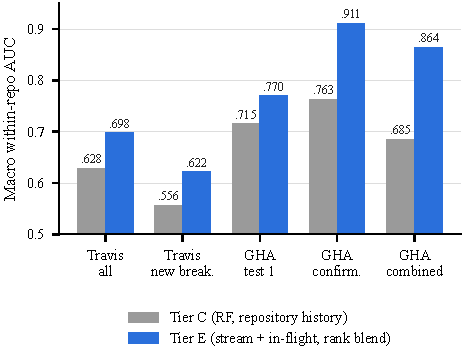
\includegraphics[width=\columnwidth]{main_results.pdf}
\caption{Macro within-repository AUC of \tierC\ (Random Forest with repository history) and \tierE\ across all evaluations (test folds; 0~h finish buffer). Travis uses folds 7--10, GitHub Actions (GHA) folds 6--10.}
\label{fig:main}
\end{figure}

\subsection{Travis~CI}
\tierE\ raises macro within-repository AUC from 0.628 to \textbf{0.698} (Table~\ref{tab:travis}), with every confirmation fold's paired CI above zero (fold \dAUC: +0.068, +0.067, +0.070, +0.074). Within-repository recall@15\% improves by +0.068. Unlike a pure persistence effect, the gain \emph{grows} as outcomes are withheld longer (Fig.~\ref{fig:buffer}): in-flight features remain informative when recent outcomes are not yet known.

\begin{table}[t]
\caption{Travis~CI, folds 7--10: macro within-repo AUC by finish buffer. Every fold's paired 95\% CI for \dAUC\ is above 0.}
\label{tab:travis}
\centering
\footnotesize
\setlength{\tabcolsep}{4pt}
\begin{tabular}{@{}rrrr@{}}
\toprule
Finish buffer & \tierC\ RF & \tierE\ blend & \dAUC \\
\midrule
0 h & 0.628 & \textbf{0.698} & +0.070 \\
1 h & 0.600 & \textbf{0.681} & +0.081 \\
6 h & 0.585 & \textbf{0.672} & +0.087 \\
\bottomrule
\end{tabular}
\end{table}

\textbf{Attribution} (Table~\ref{tab:attr}). On Travis the ranking objective is the largest single lever: it is worth +0.031 on \tierC\ features alone, and stream and in-flight features add about +0.03 more. Build-matrix size contributes only $\sim$0.003; the deployed variant omits it. The ranker trades pooled AUC for within-repository ordering: the blend's pooled AUC is 0.828 against 0.856 for \tierC\ RF. Teams that need pooled ranking should use the binary \tierE\ model, which beats \tierC\ on both metrics.

\begin{table}[t]
\caption{Attribution on Travis~CI (folds 7--10, 0~h).}
\label{tab:attr}
\centering
\footnotesize
\setlength{\tabcolsep}{4pt}
\begin{tabular}{@{}lrr@{}}
\toprule
Variant & Within-repo & Pooled \\
\midrule
\tierC, Random Forest & 0.628 & 0.856 \\
\tierC, binary LightGBM & 0.633 & -- \\
\tierC, LightGBM ranker & 0.664 & -- \\
\tierE, binary LightGBM & 0.652 & \textbf{0.881} \\
\tierE, LightGBM ranker & 0.696 & -- \\
\tierE, blend & \textbf{0.698} & 0.828 \\
\tierE, blend without job counts & 0.695 & 0.826 \\
\bottomrule
\end{tabular}
\end{table}

\subsection{New breakages}
\label{sec:newbreak}
Much of the all-builds signal comes from streams that are already failing: in folds 7--10, 55\% of failures occur on streams whose last known outcome was a failure. To check that the model does more than persistence, we rescored the saved predictions on \emph{new breakages}, builds whose previous build on the same stream passed. These are 25\% of failures, and the builds fail only 6.6\% of the time. Here the repository's last-5 failure rate is at chance (0.504), \tierC\ scores 0.556, and \tierE\ scores \textbf{0.622}. The gain (+0.066) is as large as on all builds, and every fold's CI is above zero at every buffer. The honest headline for fresh breakages is therefore $\sim$0.62, not 0.70. This analysis is post hoc.

\begin{figure}[t]
\centering
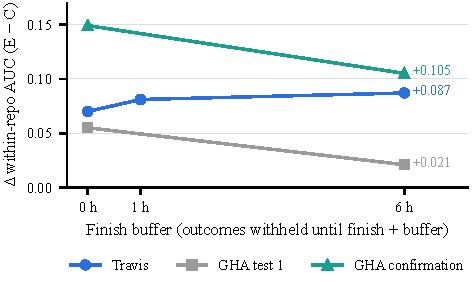
\includegraphics[width=\columnwidth]{finish_buffer.pdf}
\caption{Gain of \tierE\ over \tierC\ as outcomes are withheld longer. On Travis the gain grows; on GitHub Actions, where most runs finish within an hour, a 6~h delay removes much of the recent stream signal.}
\label{fig:buffer}
\end{figure}

\subsection{GitHub Actions: two pre-registered tests}
\label{sec:gha}
\textbf{Test 1 (30 repositories): inconclusive.} \tierE\ scored 0.770 against 0.715 (+0.055), positive in all five folds, but only 3 of 5 fold CIs excluded zero (the rule required 4), so the pre-registered verdict is \emph{inconclusive}. Recall@15\% was 0.48 against 0.37 (4 of 5 folds), and the gain shrank to +0.021 with a 6~h buffer.

\textbf{Confirmation (30 new repositories): confirms.} With every repository, the period and the protocol fresh, \tierE\ scored \textbf{0.911} against 0.763 (+0.149). All five fold CIs exclude zero, and the smallest lower bound is +0.090 (Fig.~\ref{fig:folds}, Table~\ref{tab:confirm}). Recall@15\% rose from 0.31 to 0.43 (lift 2.82$\times$ vs.\ 2.04$\times$), and \tierE\ beat \tierC\ in all 24 test repositories. The secondary analysis on both datasets combined (60 repositories) gave +0.179, again 5 of 5 folds.

\begin{figure*}[t]
\centering
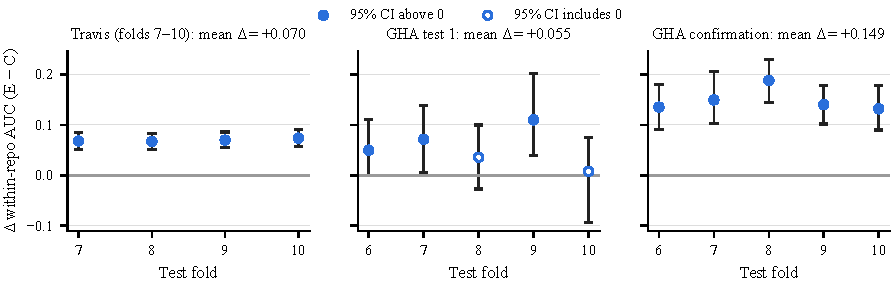
\includegraphics[width=\textwidth]{fold_deltas.pdf}
\caption{Per-fold paired \dAUC\ (\tierE\ $-$ \tierC) with repository-bootstrap 95\% CIs. Filled markers: CI excludes 0. The confirmation test meets the pre-registered rule (at least 4 of 5) in all five folds; test~1 met it in three.}
\label{fig:folds}
\end{figure*}

\begin{table}[t]
\caption{GitHub Actions confirmation (30 new repositories, folds 6--10).}
\label{tab:confirm}
\centering
\footnotesize
\setlength{\tabcolsep}{4pt}
\begin{tabular}{@{}lrrrc@{}}
\toprule
Setting & \tierC & \tierE & \dAUC & CIs $>$ 0 \\
\midrule
All runs, 0 h (primary) & 0.763 & \textbf{0.911} & +0.149 & 5/5 \\
Label-validity sensitivity & 0.765 & 0.911 & +0.147 & 5/5 \\
New breakages, 0 h & 0.642 & 0.683 & +0.041 & 2/5 \\
All runs, 6 h buffer & 0.741 & 0.846 & +0.105 & 5/5 \\
New breakages, 6 h & 0.637 & 0.634 & $-$0.004 & 0/5 \\
\midrule
Combined, 60 repos (secondary) & 0.685 & 0.864 & +0.179 & 5/5 \\
\bottomrule
\end{tabular}
\end{table}

\textbf{Is it only ``it failed last time''?} The confirmation gain is nearly three times test~1's, and failures are three times as common. We therefore checked a naive persistence score: whether the stream's previous finished run failed. It reaches only $\sim$0.72, below \tierC\ (Fig.~\ref{fig:persist}), and the per-repository gain is uncorrelated with the repository's failure rate ($r=0.03$). This check was exploratory, not pre-registered.

\begin{figure}[t]
\centering
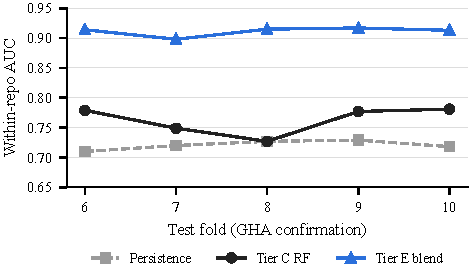
\includegraphics[width=\columnwidth]{persistence.pdf}
\caption{Confirmation test: \tierE\ against \tierC\ and a naive stream-persistence score (exploratory).}
\label{fig:persist}
\end{figure}

\textbf{What differs from Travis.} On GitHub Actions the stream and in-flight features carry the gain; the ranking objective alone adds only +0.010 (test~1) and +0.042 (confirmation). Most runs finish within an hour, so the very recent outcome of the same stream is the key signal, and withholding it for 6~h removes most of the new-breakage gain. The size of the gain varies by project (+0.055 to +0.149); the consistent finding is its sign.

\subsection{Negative results}
Adding repository-level streak and gap features to \tierC\ \emph{reduced} within-repository AUC by 0.019 (4 of 5 folds significantly). Streaks that mix all of a repository's branches are noise; per-stream history is the version of this idea that helps.

%=====================================================================
\section{Deployed System}
\label{sec:system}
%=====================================================================

\begin{figure}[t]
\centering
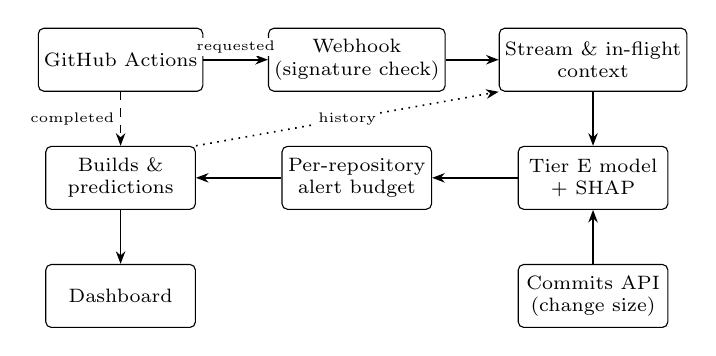
\begin{tikzpicture}[
  font=\scriptsize,
  box/.style={draw, rounded corners=2pt, align=center, minimum height=8mm, minimum width=19mm, inner sep=2pt, fill=white},
  arr/.style={-{Stealth[length=1.6mm]}, semithick},
  lab/.style={font=\tiny, fill=white, inner sep=1pt}]
\node[box] (gh)    at (0, 0)     {GitHub Actions};
\node[box] (hook)  at (3.0, 0)   {Webhook\\(signature check)};
\node[box] (ctx)   at (6.0, 0)   {Stream \& in-flight\\context};
\node[box] (db)    at (0, -1.5)  {Builds \&\\predictions};
\node[box] (alert) at (3.0, -1.5){Per-repository\\alert budget};
\node[box] (model) at (6.0, -1.5){\tierE\ model\\+ SHAP};
\node[box] (ui)    at (0, -3.0)  {Dashboard};
\node[box] (cmt)   at (6.0, -3.0){Commits API\\(change size)};
\draw[arr] (gh) -- node[lab, above=1pt] {requested} (hook);
\draw[arr] (hook) -- (ctx);
\draw[arr] (ctx) -- (model);
\draw[arr] (model) -- (alert);
\draw[arr] (alert) -- (db);
\draw[arr] (db) -- (ui);
\draw[arr] (cmt) -- (model);
\draw[arr, dashed] (gh) -- node[lab, left=1pt] {completed} (db);
\draw[arr, dotted] (db.north east) -- node[lab] {history} (ctx.south west);
\end{tikzpicture}
\caption{Scoring path. A \emph{requested} workflow run is scored before it executes; its \emph{completed} event attaches the real outcome, which becomes history for later runs. Nothing blocks CI.}
\label{fig:arch}
\end{figure}

\textbf{Architecture} (Fig.~\ref{fig:arch}). A FastAPI service receives signed GitHub \texttt{workflow\_run} events. When a run is \emph{requested}, the service builds its stream history and in-flight context from the repository's stored runs and fetches its commit's size. It then scores the run with the \tierE\ model, trained on folds 1--9 of the 146{,}556 GitHub Actions runs, and stores a shadow prediction. When the run \emph{completes}, its outcome is attached. Other conclusions, such as \texttt{cancelled}, are stored but never become history, mirroring training. Runs are timed by GitHub's own \texttt{created\_at} and \texttt{updated\_at}, so a late webhook delivery does not change a run's history. Tests check that the live history equals the offline training pass row by row. The deployed artifact reproduces the research fold-10 predictions exactly, with a maximum difference of 0. On that holdout its within-repository AUC is 0.913, and 0.893 with all workflow identities treated as unseen, as for a newly connected repository.

\textbf{Per-repository alert budget.} A single global threshold does not implement the evaluated metric. Taken as the 85th percentile of the holdout, which was 36\% failures, it sat at 0.94 and flagged between 3\% and 51\% of a repository's runs. Alerts instead follow the evaluation: a run is flagged when its risk reaches the 85th percentile of its repository's last 100 scored runs. Until a repository has 20 scored runs, it uses a ``typical repository'' threshold: the median, over holdout repositories, of each one's 85th percentile. Neither threshold uses labels. Replayed in time order on the holdout (Fig.~\ref{fig:alert}, Table~\ref{tab:alert}), each repository flags 11--22\% of its runs, and the mean share of a repository's failures caught rises from 34\% to 41\%, close to the 43\% measured in hindsight. Pooled precision falls (0.80 vs.\ 0.97) only because the global threshold spends nearly all its alerts on the repositories that fail most.

\begin{figure}[t]
\centering
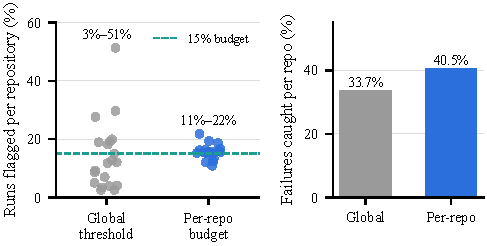
\includegraphics[width=\columnwidth]{alert_policy.pdf}
\caption{Deployed model's holdout: share of each repository's runs flagged (left; one dot per repository) and mean share of a repository's failures caught (right), for one global threshold and for the per-repository budget.}
\label{fig:alert}
\end{figure}

\begin{table}[t]
\caption{Alert policies on the deployed model's holdout (20 repositories).}
\label{tab:alert}
\centering
\footnotesize
\setlength{\tabcolsep}{4pt}
\begin{tabular}{@{}lrr@{}}
\toprule
& Global (0.94) & Per-repo budget \\
\midrule
Runs flagged per repository & 3--51\% & 11--22\% \\
Failures caught per repository (mean) & 34\% & \textbf{41\%} \\
Pooled precision of alerts & 0.97 & 0.80 \\
\bottomrule
\end{tabular}
\end{table}

\textbf{Dashboard and public demonstration.} A React dashboard shows risk trends, the risk distribution, model evidence (Fig.~\ref{fig:dash}), and per-repository risk timelines with real outcomes (Fig.~\ref{fig:timeline}). It also lets users score a run with the history the server derives (Fig.~\ref{fig:submit}) and explore what-if changes with SHAP explanations (Fig.~\ref{fig:whatif}). A read-only public deployment replays 450 real runs from \texttt{twbs/bootstrap}, \texttt{freeCodeCamp} and \texttt{yt-dlp} through the real webhook, at their real GitHub times. The runs come from the model's holdout window and were never trained on. PR authors and branch names are pseudonymised. Its within-repository AUCs (0.80, 0.95, 0.74) are close to the research evaluation of the same runs (0.78, 0.97, 0.79). The remaining gap comes from the demonstration starting each repository with empty history.

\begin{figure*}[t]
\centering
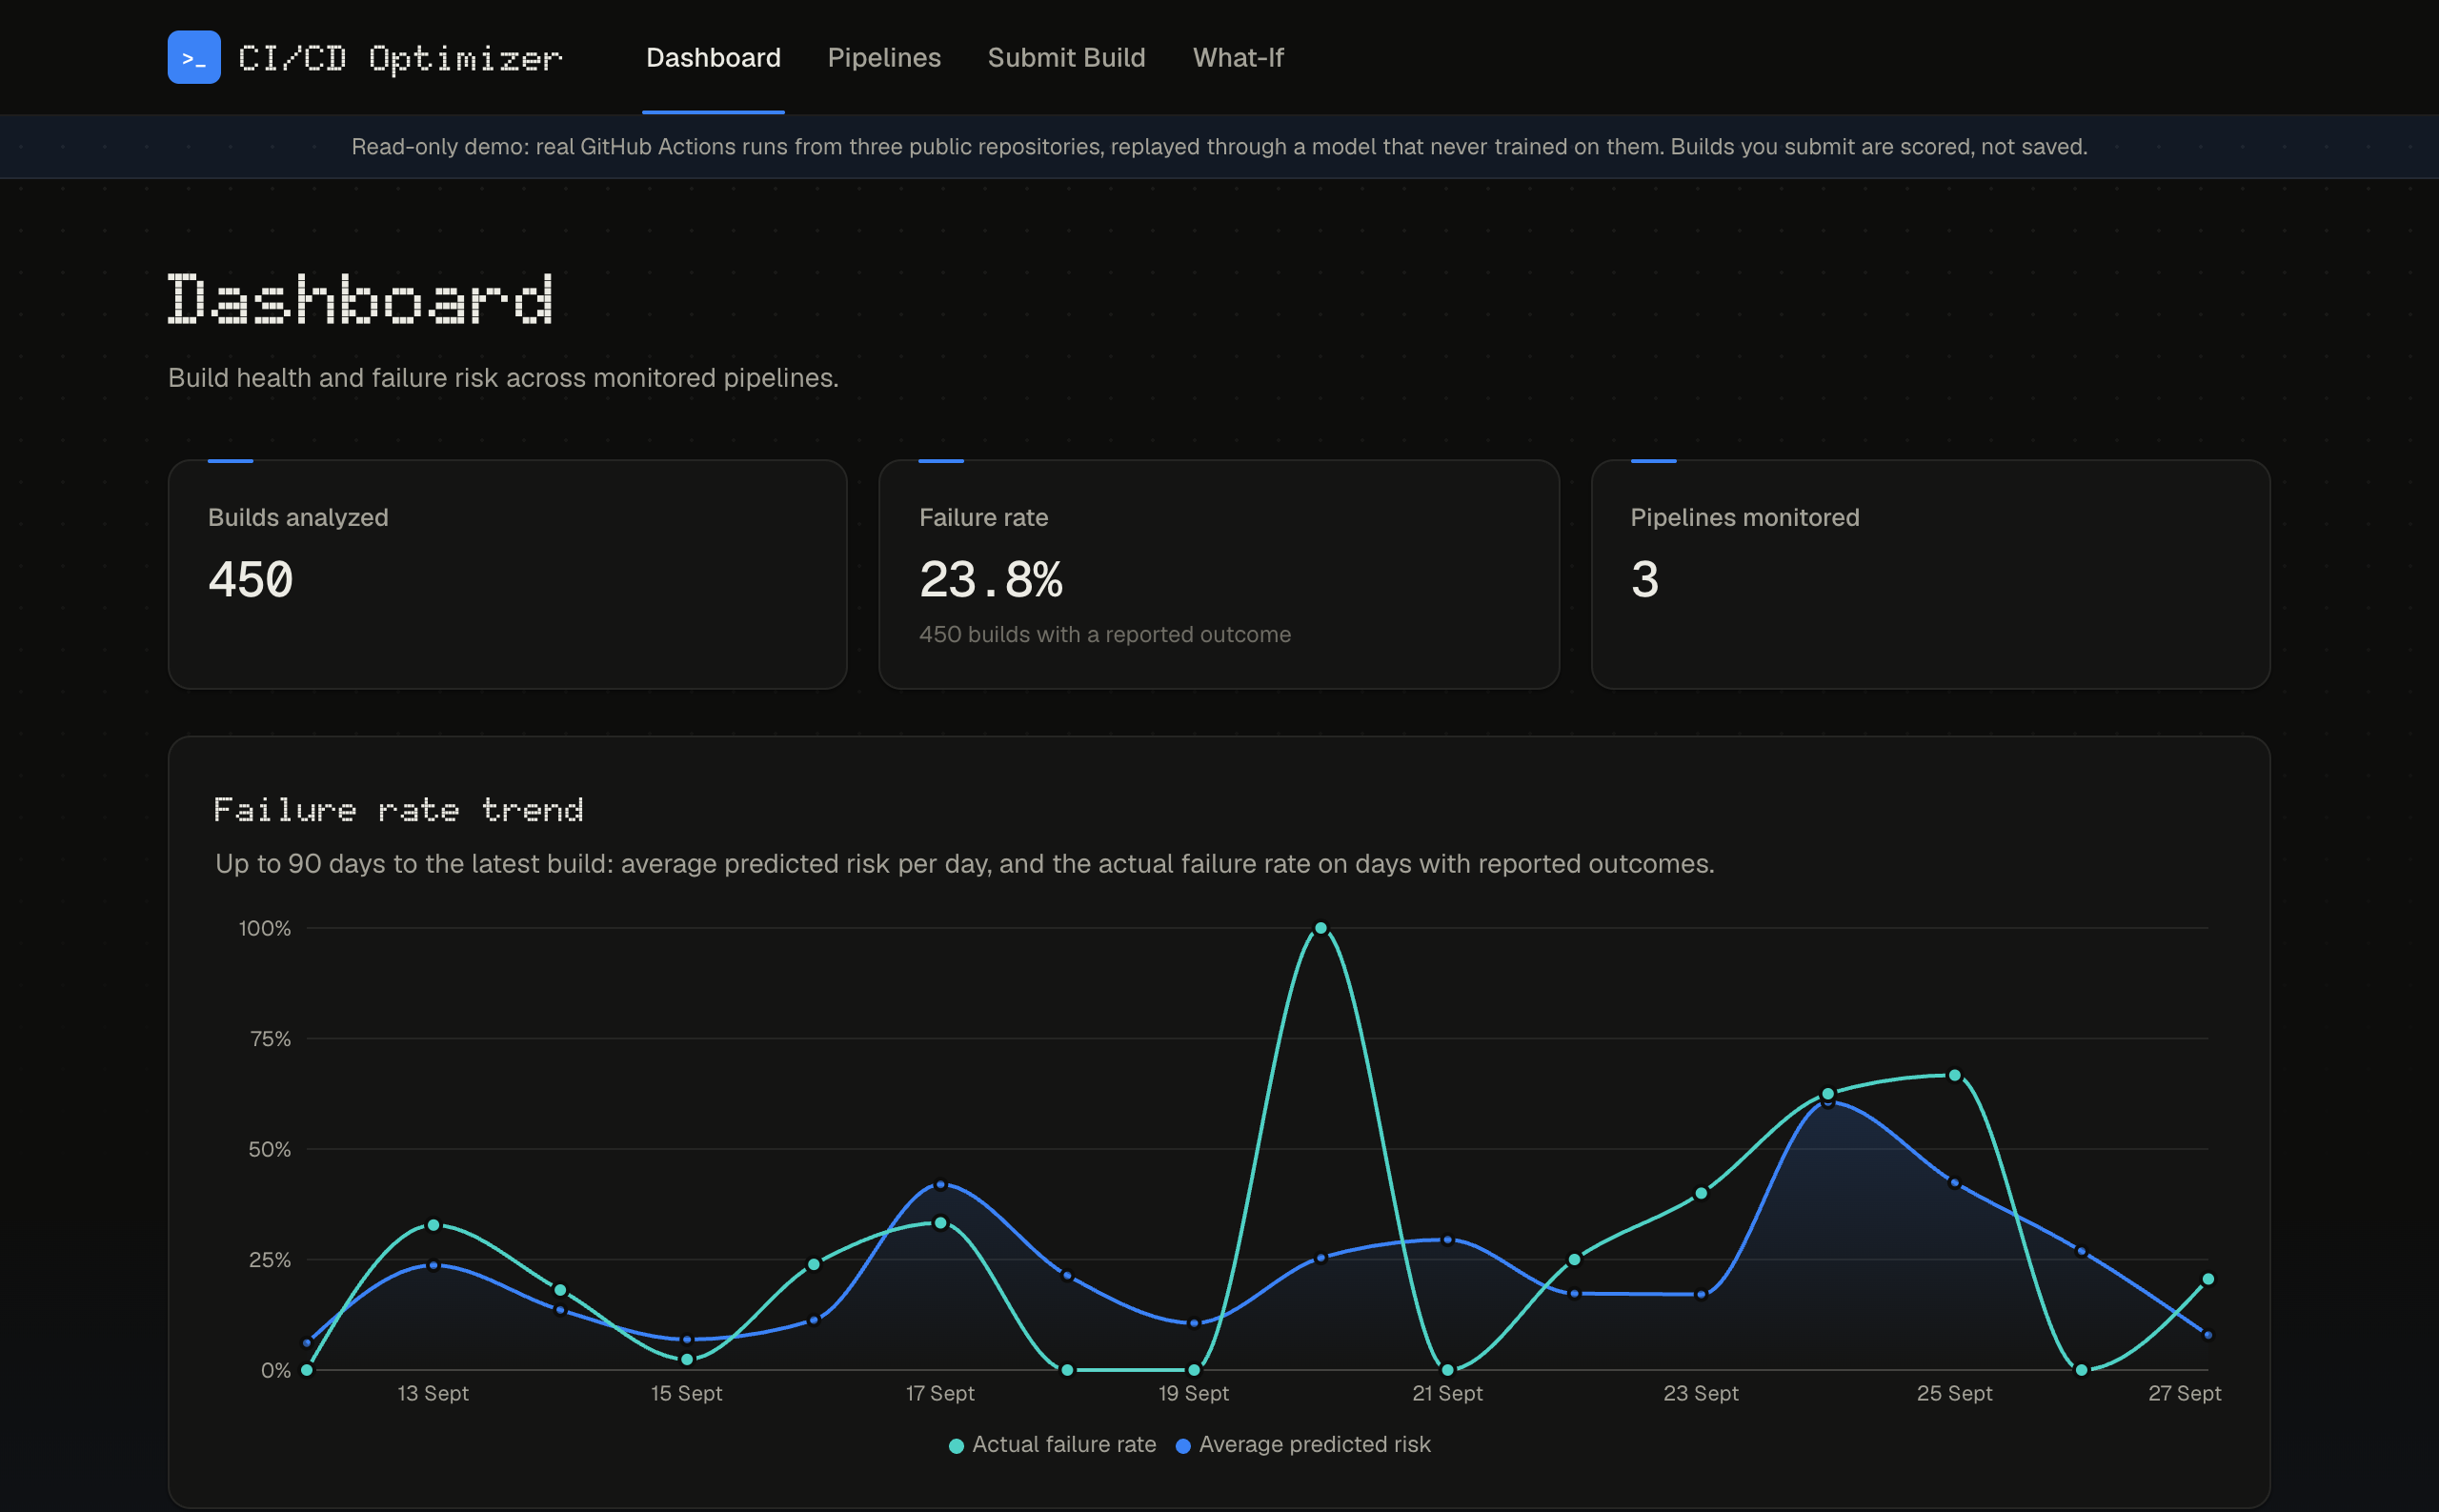
\includegraphics[height=4.75cm]{dashboard_overview.png}\hfill
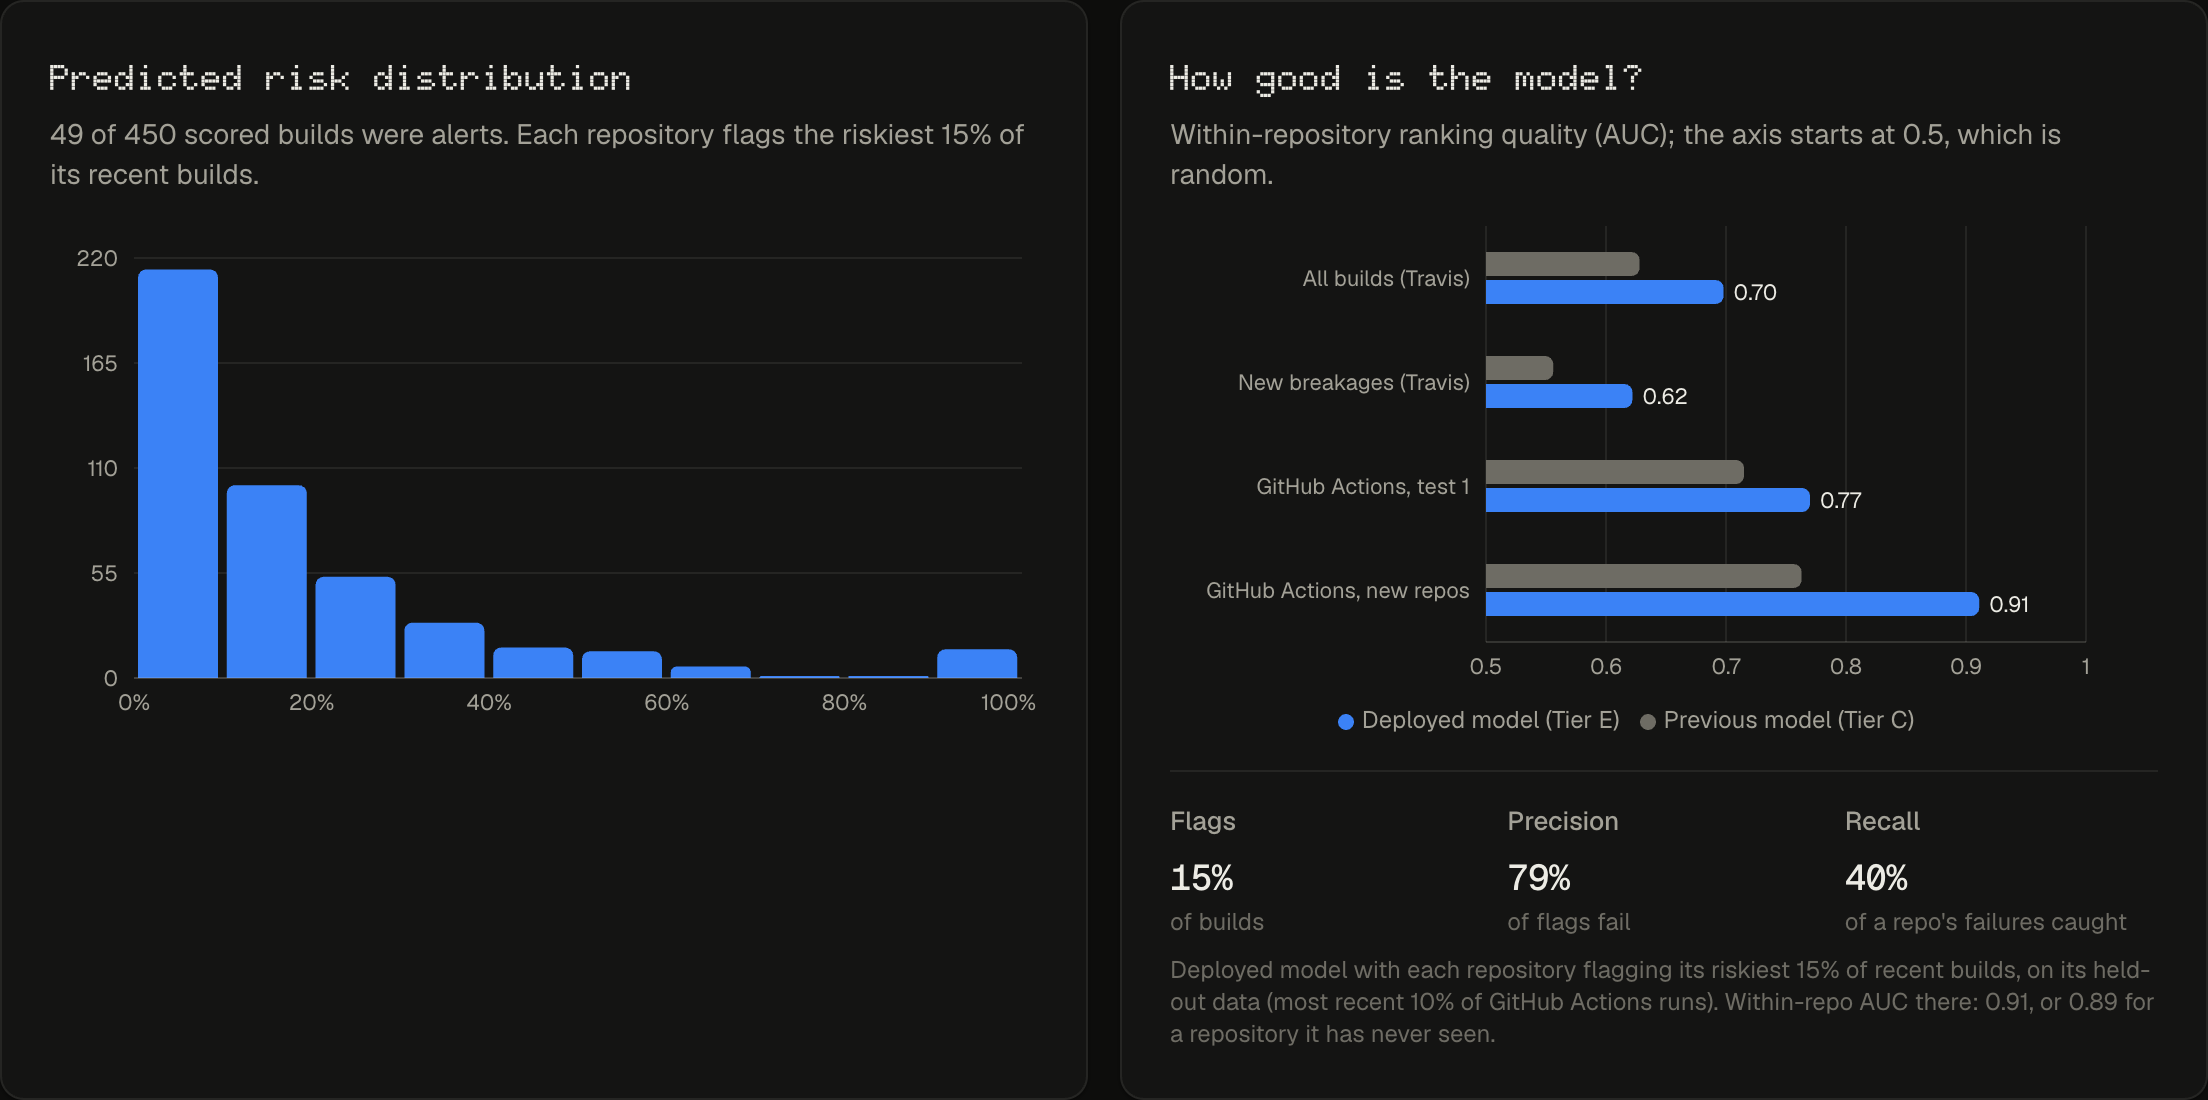
\includegraphics[height=4.75cm]{dashboard_models.png}
\caption{Dashboard of the public demonstration. Left: summary and daily failure-rate trend; average predicted risk tracks the actual failure rate. Right: risk distribution of the 450 scored runs (49 alerts under the per-repository budget) and the model-evidence panel with the research results and the deployed model's holdout statistics.}
\label{fig:dash}
\end{figure*}

\begin{figure}[t]
\centering
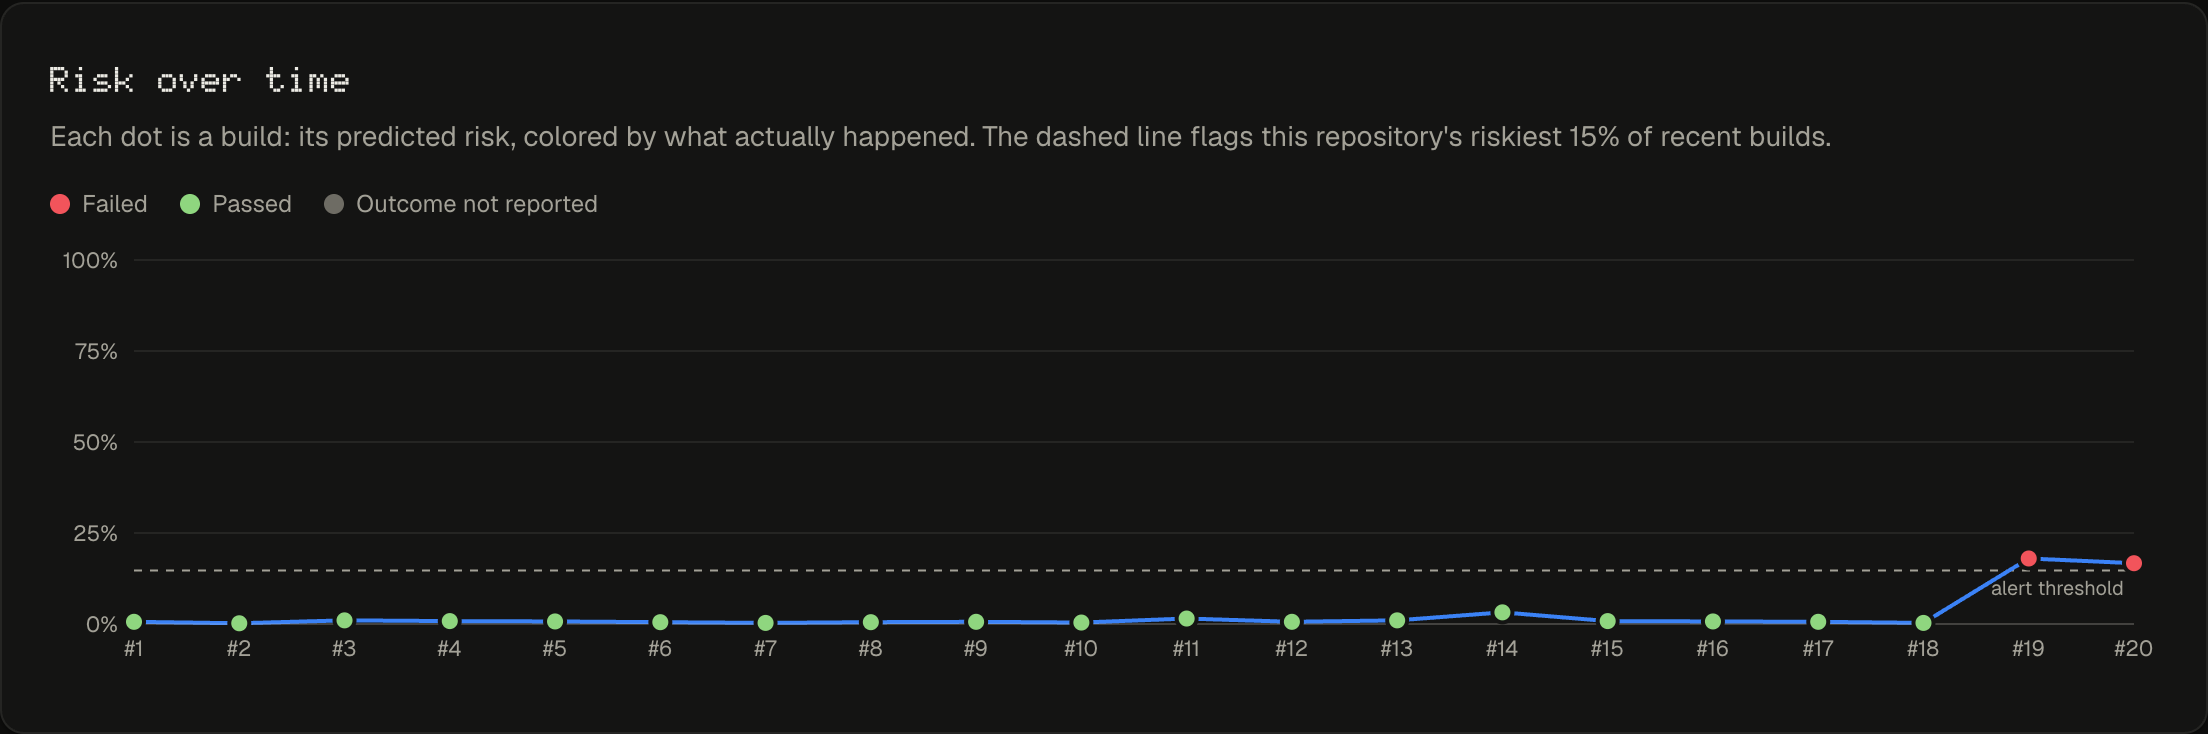
\includegraphics[width=\columnwidth]{pipeline_timeline.png}
\caption{Risk timeline for \texttt{twbs/bootstrap}: each dot is a run, coloured by its real outcome. The dashed line is this repository's alert threshold under its 15\% budget. The two newest runs, both real failures, rise above it.}
\label{fig:timeline}
\end{figure}

\begin{figure}[t]
\centering
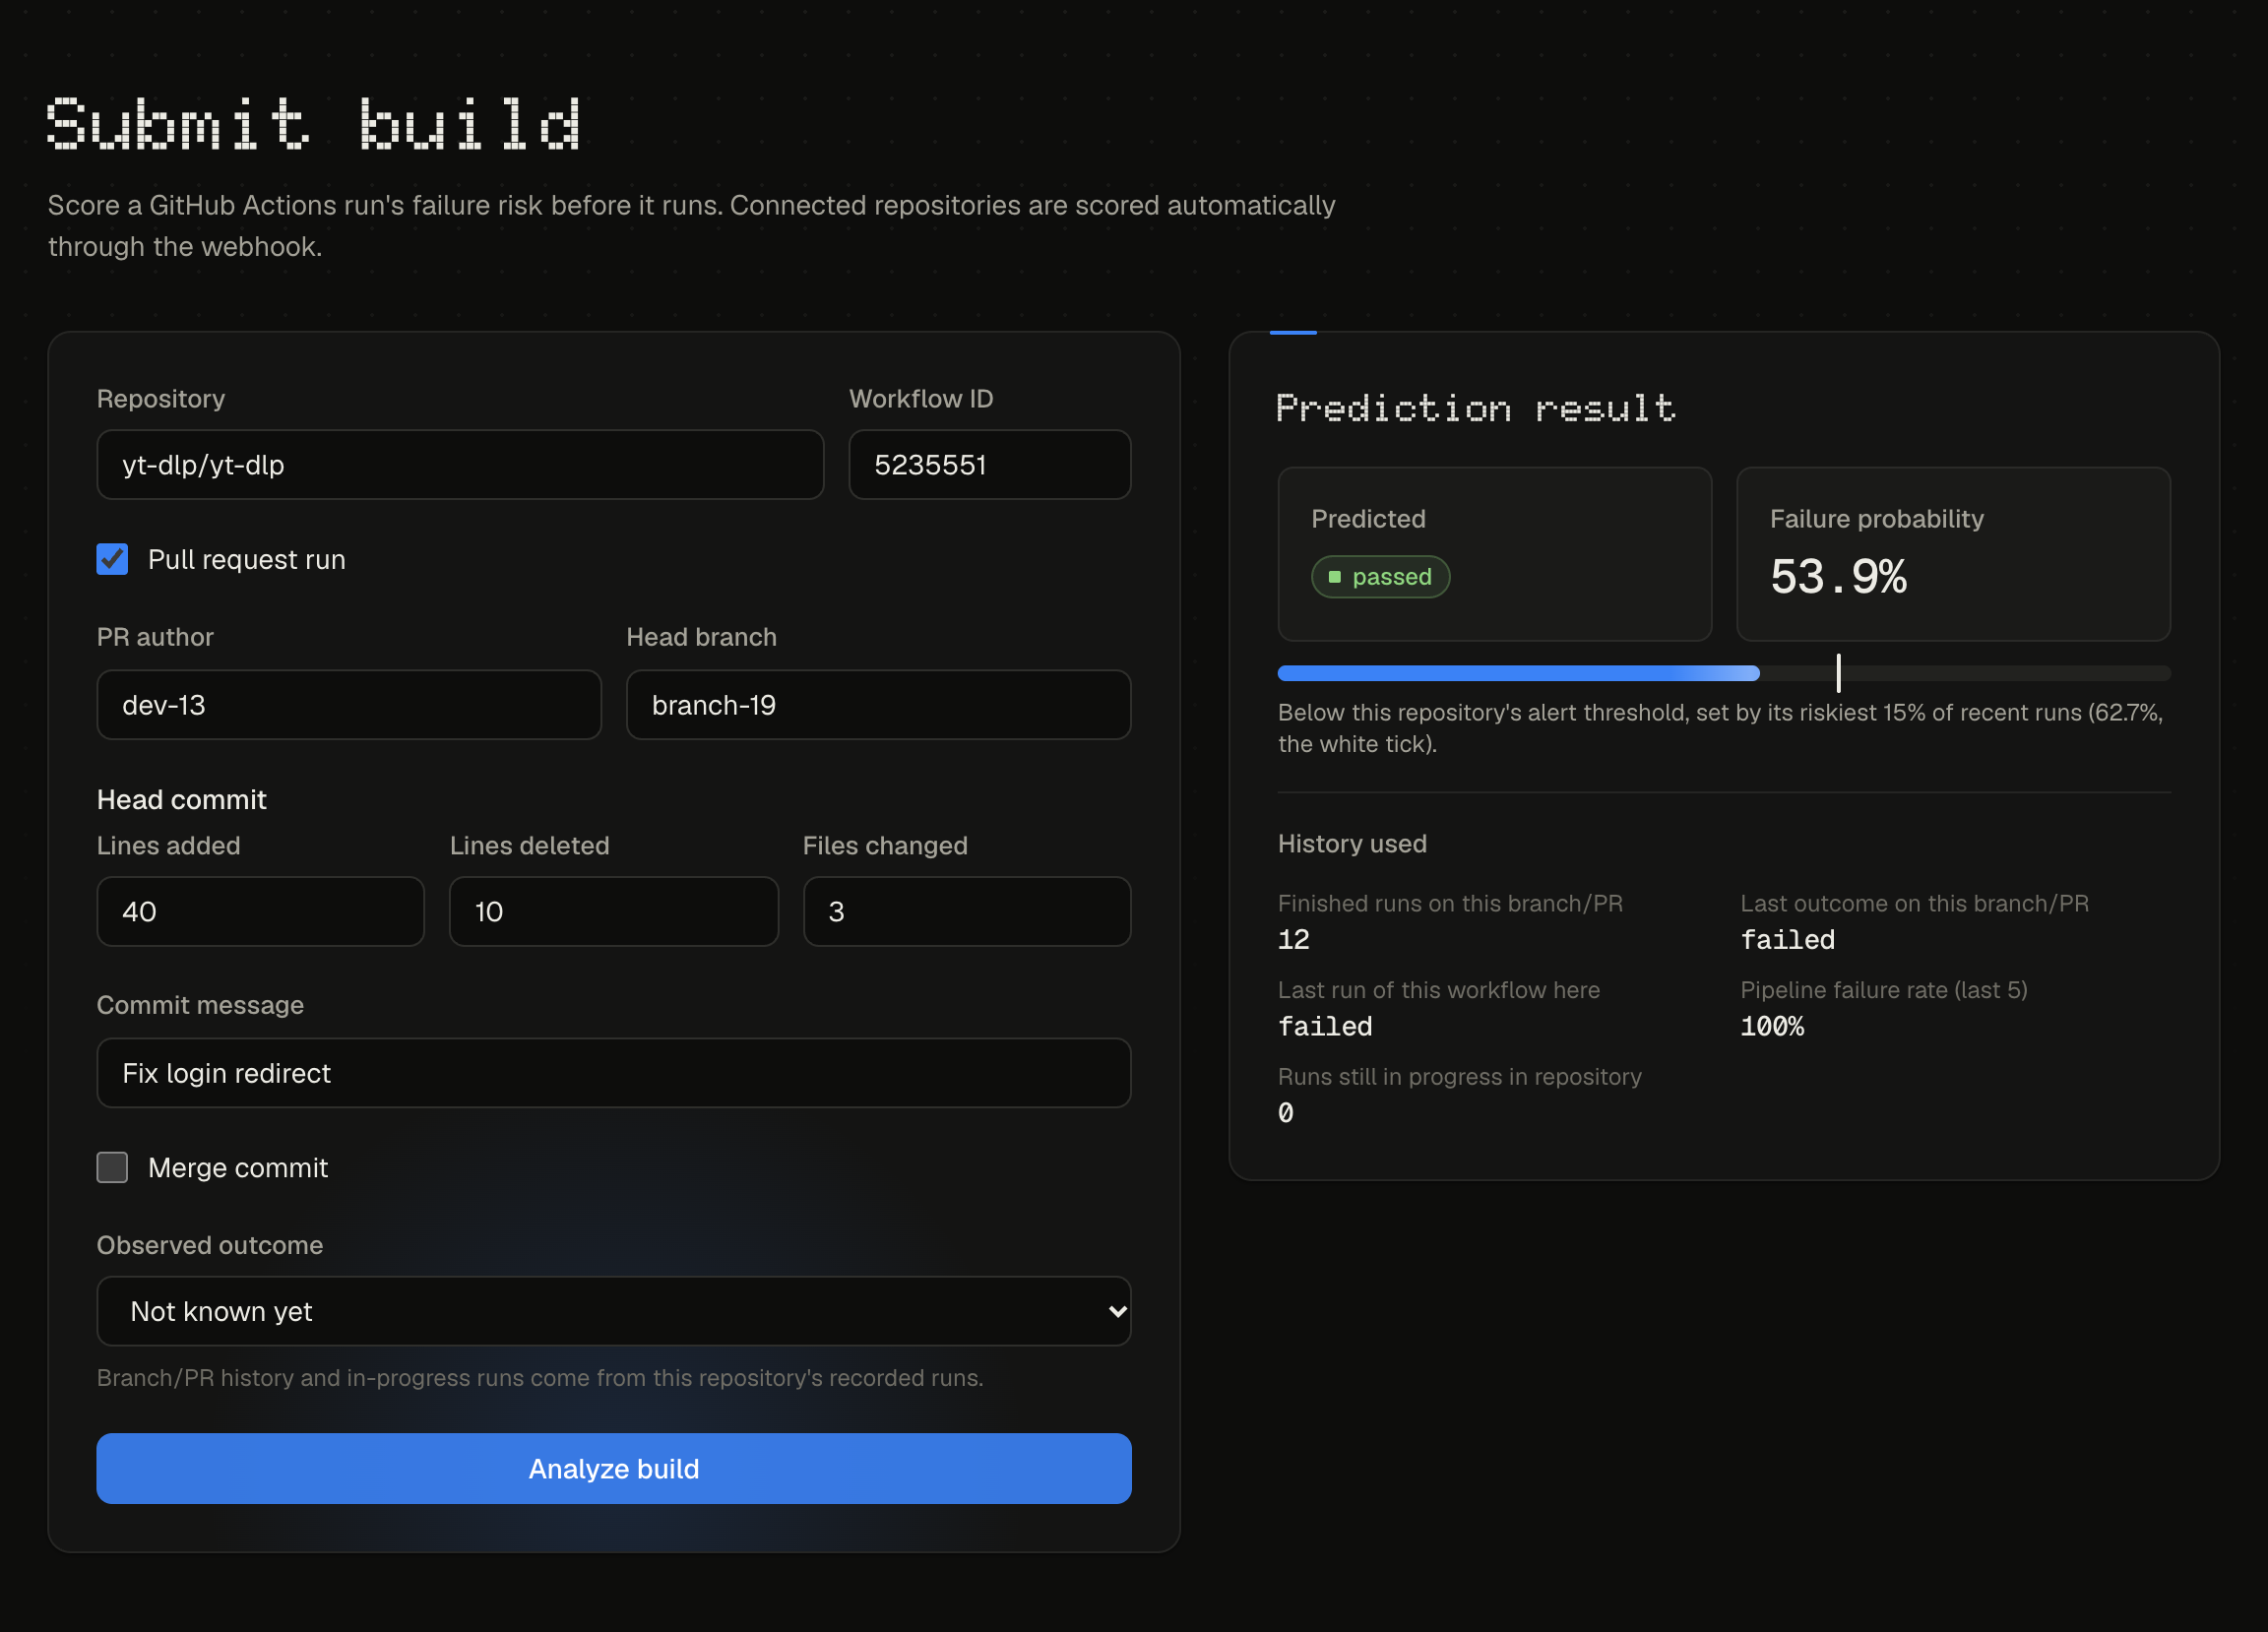
\includegraphics[width=\columnwidth]{submit_result.png}
\caption{Scoring a pull-request run on a failing \texttt{yt-dlp} stream. The server derives the history (12 finished runs, last one failed) and compares the risk with the repository's own alert threshold.}
\label{fig:submit}
\end{figure}

\begin{figure}[t]
\centering
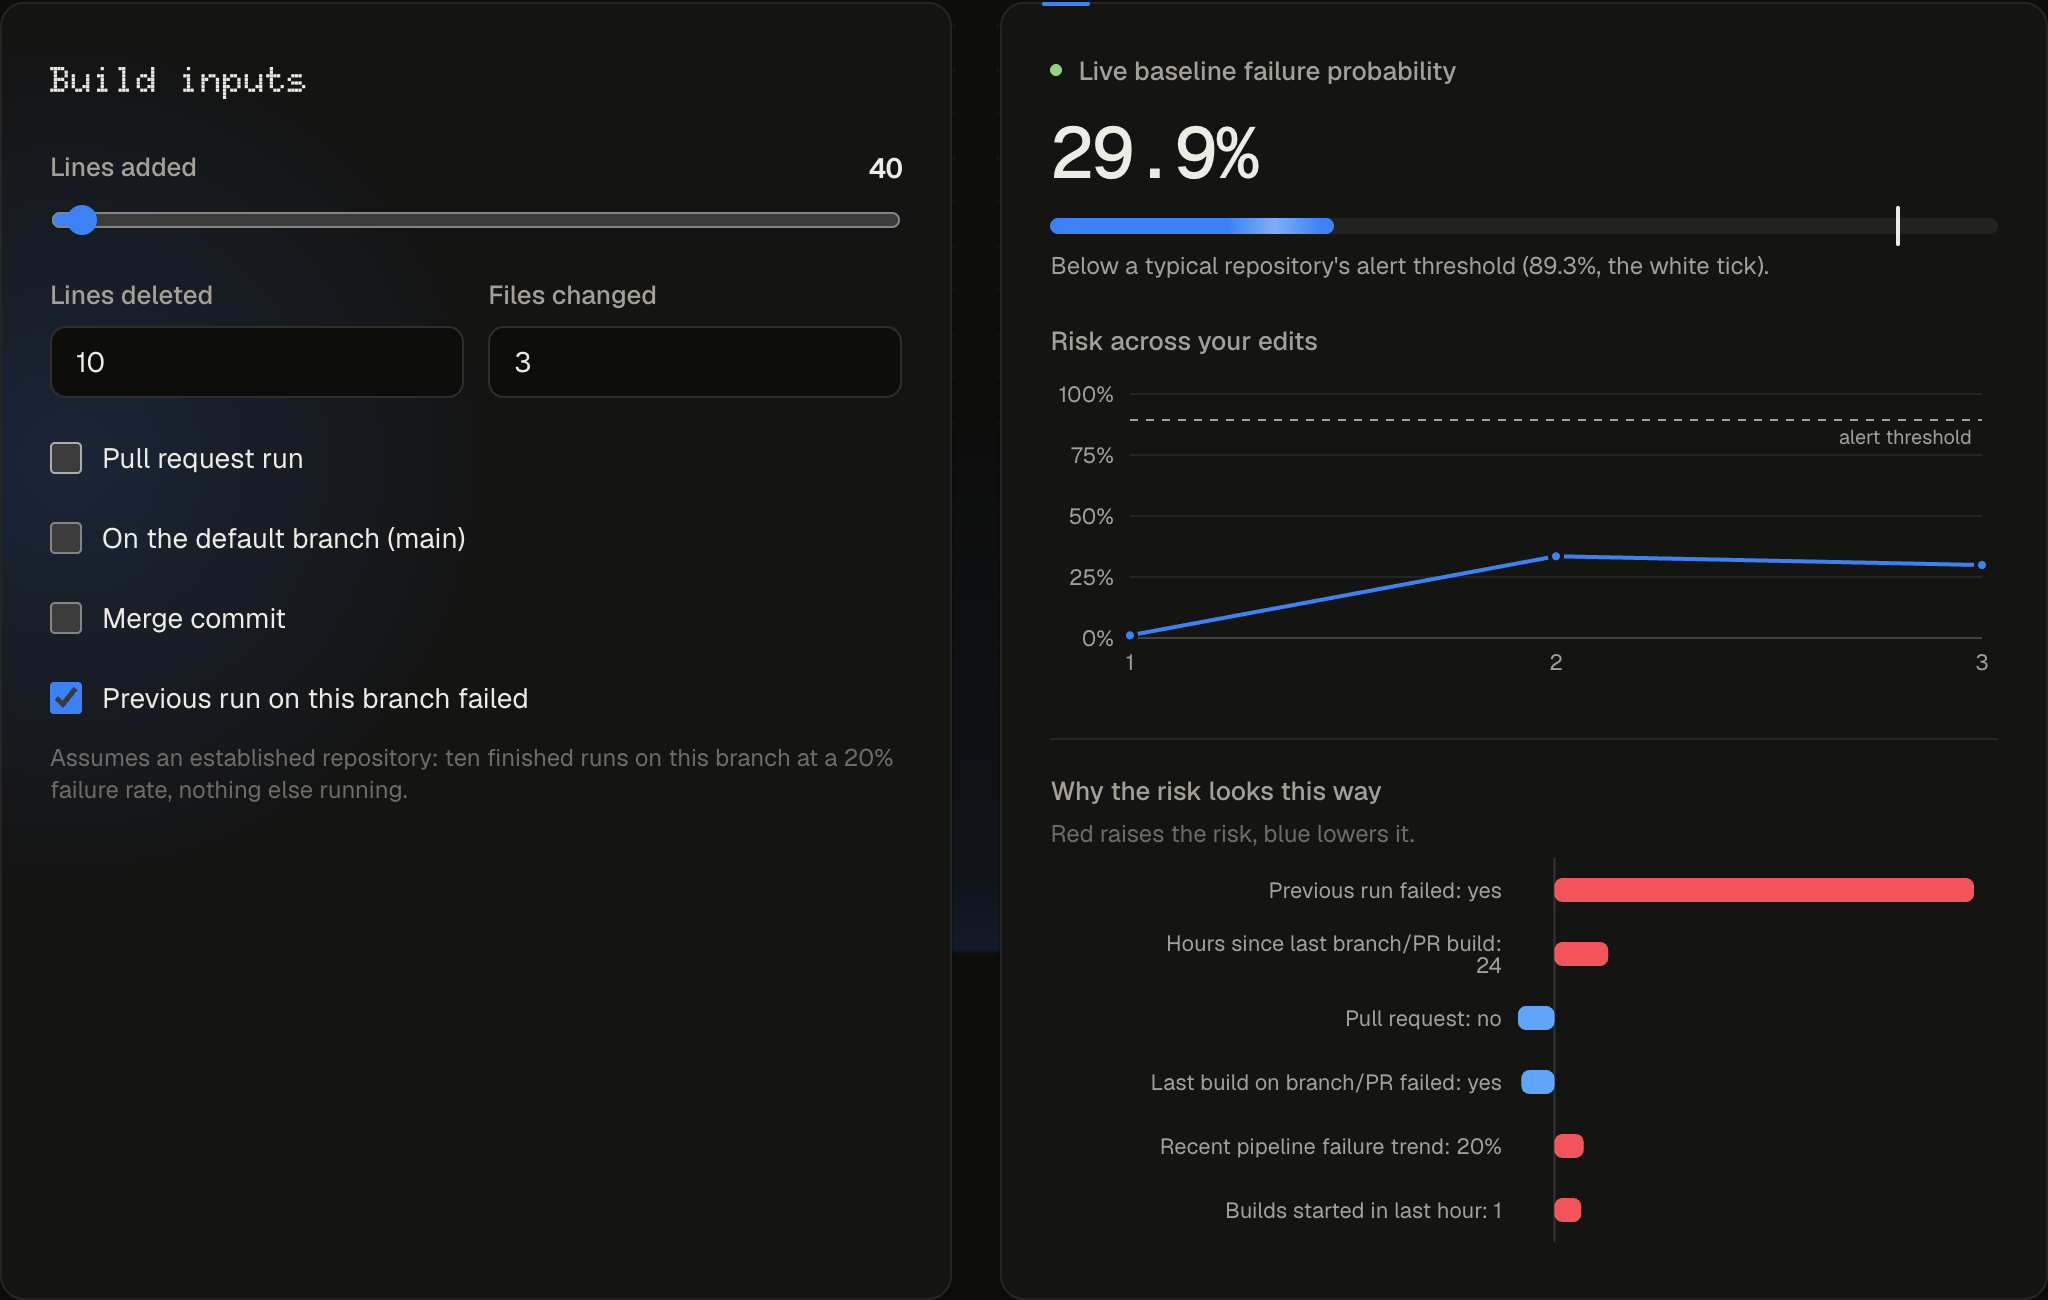
\includegraphics[width=\columnwidth]{what_if.png}
\caption{What-if page: SHAP contributions of the binary half explain the live risk. Here, whether the previous run of the same workflow failed dominates.}
\label{fig:whatif}
\end{figure}

%=====================================================================
\section{Threats to Validity}
%=====================================================================

\textbf{Internal.} The new-breakage analysis and the persistence check are post hoc. Travis fold~6 was used for development, so only folds 7--10 are confirmatory. Finish times on Travis are derived from job durations with a fallback. On GitHub Actions, 4.6\% of confirmation runs were lost to unfetchable fork commits, and these runs failed more often (38.5\% vs.\ 28.2\%).

\textbf{External.} Repositories come from popular open-source projects. In the confirmation data, the cap of the earliest 4{,}000 runs per repository left six of the busiest projects in training folds only. The gain's size varies widely by project; we claim its sign, not a fixed size.

\textbf{Construct.} Within-repository AUC measures ranking, not calibrated risk. Recall at a 15\% budget assumes teams review a fixed share of builds. A run on GitHub Actions is one workflow, so one push yields several runs that share history.

%=====================================================================
\section{Pre-Registered Forward-Looking Test}
\label{sec:prospective}
%=====================================================================

All results above test the \emph{recipe} on data that already existed. To test the \emph{deployed system}, we pre-registered a forward-looking evaluation before collecting any of its data. It scores October~2026 runs from the 60 training repositories, collected no earlier than 28~November~2026, with the frozen model (artifact SHA-256 \texttt{57c26f17\ldots}) and the frozen alert rule. History starts empty on 1~October, exactly as if the service had been connected then. Each repository's first 25\% of runs serves as warm-up and is not evaluated. The primary result is the macro within-repository AUC against a stream-persistence baseline, with a repository-bootstrap CI. The system ``holds up'' if the lower CI bound is above zero \emph{and} the AUC is at least 0.80. The protocol, repository list, and fingerprints of the frozen code are committed with the project.

%=====================================================================
\section{Conclusion}
%=====================================================================

Build failure prediction looks far easier than it is when leaky fields, random splits, or pooled metrics are allowed: on Travis~CI, an AUC of 0.91 shrinks to 0.63 under a protocol that matches a team's decision. Within that protocol, stream-level history, in-flight context, and a ranking objective improve within-repository ranking on Travis~CI (0.628 to 0.698, and 0.556 to 0.622 on new breakages). The gain carried over to GitHub Actions, where a pre-registered confirmation on 30 new repositories met its decision rule in every fold. Deployed with a per-repository review budget, the model catches about 41\% of a repository's failures in its riskiest 15\% of runs. The forward-looking test will show whether the frozen system holds up on data that did not exist when it was built.

\section*{Availability}
Code, protocols, and results: \url{https://github.com/yasaswinipakam/cicd-ai-optimizer}. Read-only demonstration: \url{https://cicd-ai-optimizer.onrender.com}.

\bibliographystyle{IEEEtran}
\bibliography{refs}

\end{document}
